% ========================================
\section{Numerical experiments}\label{sec:Num-Exp}
% ========================================
%
We present numerical results for both Monte Carlo and multi-fidelity Monte Carlo sampling methods to estimate the expectation $\mathbb{E}(u)$. Following \cite{FaHe:2017}, the computational framework is built upon an ITER reactor geometry featuring twelve magnetic coils, with the \textit{reference currents} $\boldsymbol{I}$ specified as
%
\begin{equation}\label{eq:CentralCurrentValue}
{\renewcommand{\arraycolsep}{2pt}
\begin{array}{llll}
I_1 = -1.4 \times 10^{6} A, \quad & I_2 = -9.5 \times 10^{6} A, \quad & I_3 = -2.0388 \times 10^{7} A, \quad & I_4 = -2.0388 \times 10^{7} A, \\
I_5 = -9 \times 10^{6} A, \quad & I_6 = 3.564 \times 10^{6} A, \quad & I_7 = 5.469 \times 10^{6} A, \quad & I_8 = -2.266 \times 10^{6} A, \\
I_9 = -6.426 \times 10^{6} A, \quad & I_{10} = -4.82 \times 10^{6} A, \quad & I_{11} = -7.504 \times 10^{6} A, \quad & I_{12} = 1.724 \times 10^{7} A. 
\end{array}
}
\end{equation}
%
The profiles for $p$ and $g$ on the right-hand side of \eqref{eq:FreeBoundary} follow the form given in \eqref{eq:source}, using the following \textit{reference parameter} values
%
\begin{equation}\label{eq:CentralParameterValue}
r_0=6.2m,\,\,\beta=0.5978, \,\, \alpha_1 = 2, \,\,  \alpha_2=1.395, \,\, j_0=1.3655 \times 10^6 A/m^2,\,\,  \mu_0=1.2566\times 10^{-6} N/A^2.
\end{equation}
%
To evaluate the sensitivity of the solution to \eqref{eq:FreeBoundary} under uncertainty, we conduct two experiments, each introducing a specific source of variability. In the first experiment, uncertainties are introduced in the coil currents, modeled as uniformly distributed perturbations of $\tau = 2\%$ around the reference currents in \eqref{eq:CentralCurrentValue}, while the profile parameters are held fixed at their reference values, isolating the impact of current variability on the solution.  In the second experiment, uncertainties are introduced in the profile parameters, modeled as uniformly distributed perturbations of $\tau = 1\%$ around the reference values in \eqref{eq:CentralParameterValue}, with the coil currents kept constant. The reactor geometry and coil arrangement adhere to the descriptions provided in \cite{Amoskov:2009}.  A family of nested spatial meshes $\{\mathcal{T}_k\}$ is generated by refining and coarsening the reference ITER geometry, yielding six distinct spatial discretizations, with the number of spatial grid nodes $\{M_\ell,\}_{0\le \ell \le 5}$  satisfying
%
\begin{equation}
\label{eq:MeshGrowth}
M_\ell = s M_{\ell-1} \qquad \text{ for } s>1.
\end{equation}
%
The number of the available spatial grid nodes are shown in the first row of Table \ref{Tab:Dof}.



The splitting ratio $\theta$ is set to 0.5 to reflect a balance between discretization and statistical errors. Tolerances for the normalized mean square error are chosen to slightly exceed the discretization error on the finest available mesh $(\ell=5)$, with values $\epsilon=2\times 10^{-4}, 4\times 10^{-4}, 6\times 10^{-4}, 8\times 10^{-4}, 1\times 10^{-3}, 2\times 10^{-3}, 4\times 10^{-3}, 8\times 10^{-3}$. Based on these tolerances, the corresponding spatial grid levels required to meet the discretization error thresholds are determined using the relation outlined in \eqref{eq:SLSGC_MLS_SpatialGridsNo}, resulting in levels $L = 5, 4, 4, 4, 4, 3, 3, 2, 2$. To ensure numerical stability in computing the sample mean, variance and covariance,  Welford's algorithm \cite{Welford:1962} is used for both high- and low-fidelity models, ensuring robust online computation of the statistics. For the high-fidelity model, denoted as $\widehat u_{h,1}=u_h$, the iterative updates to the sample mean and variance are 
%
\[
m_w^{(i)} = m_w^{(i-1)} + \frac{u_h\left(\boldsymbol{\omega}^{(i)}\right)-m_w^{(i-1)}}{i},\qquad s_w^{(i)} = s_w^{(i-1)} + \left\langle u_h\left(\boldsymbol{\omega}^{(i)}\right)-m_w^{(i-1)}, \;\;u_h\left(\boldsymbol{\omega}^{(i)}\right)-m_w^{(i)}\right\rangle,
\]
%
Similarly, for the low-fidelity model $\widehat u_{h,k}$, the mean and variance are updated as
%
\[
\widehat m_w^{(i)} = \widehat m_w^{(i-1)} + \frac{\widehat u_{h,k}\left(\boldsymbol{\omega}^{(i)}\right) - \widehat m_w^{(i-1)}}{i},\qquad \widehat s_w^{(i)} = \widehat s_w^{(i-1)} + \left\langle \widehat u_{h,k}\left(\boldsymbol{\omega}^{(i)}\right)-\widehat m_w^{(i-1)},\;\; \widehat u_{h,k}\left(\boldsymbol{\omega}^{(i)}\right)-\widehat m_w^{(i)}\right\rangle,
\]
%
The covariance between the high- and low-fidelity models is computed using
%
\[
v_w^{(i)} = v_w^{(i-1)} + \left \langle u_{h}\left(\boldsymbol{\omega}^{(i)}\right)-m_{w}^{(i-1)},\;\;\widehat u_{h,k}\left(\boldsymbol{\omega}^{(i)}\right)-\widehat m_{w}^{(i-1)}\right\rangle.
\]
%

Experiments were performed using MATLAB R2024a on the batch-scheduled HPC/HTC cluster NOTSx, part of the Rice Big Research Data cloud infrastructure. The system consists of 298 dual-socket compute blades housed on HPE s6500, HPE Apollo 2000, and Dell PowerEdge C6400 chassis. All nodes are interconnected via a high-speed network with 10 or 25 Gigabit Ethernet.


% =============================
\subsection{Uncertainties in the currents}
% =============================
In this experiment, we study the uncertainty in perturbing the baseline currents \eqref{eq:CentralCurrentValue} in the twelve coils. 



The high-fidelity model for each tolerance corresponds to the finite element solution of \eqref{eq:FreeBoundary} that achieves the specified discretization accuracy with level $L$.  To construct the low-fidelity models, we consider to use sparse grid stochastic collocation to build interpolations following \eqref{eq: Smolyak_Quad_formula} for the high fidelity models with level $q=1$ sparse grid nodes \eqref{eq:NestedColPts} in the parameter space. Moreover, for each tolerance, we select the candidate low-fidelity models such that they are built over a sequence of spatial meshes with number of grid nodes smaller than or equal to those of the corresponding high-fidelity model. Table \ref{Tab:Time_build_surrogate_est_para} shows the computational cost to build surrogates for each tolerance $\epsilon$ and estimate the parameters required to perform the muli-fidelity Monte Carlo.





%
\begin{table}[ht]
\centering
\scalebox{0.8}{
\begin{tabular}{c|c|c|c|c|c|c|c|c|c|c|c|c|c|c|c|c|c|c|}
\hline
\multicolumn{1}{|c|}{$\epsilon$} &$8\times 10^{-3}$&$6\times 10^{-3}$&$4\times 10^{-3}$&$2\times 10^{-3}$&$10^{-3}$&$8\times 10^{-4}$&$6\times 10^{-4}$&$4\times 10^{-4}$&$2\times 10^{-4}$\\
\hline
\multicolumn{1}{|c|}{Build surrogate }&2.11e+01&2.11e+01&1.08e+02&1.08e+02&5.53e+02&5.53e+02&5.53e+02&5.53e+02&2.39e+03\\
\hline
\multicolumn{1}{|c|}{Estimate parameters}&&&&&&&&\\
% &2.02e+00&7.90e+00&3.10e+01&1.52e+02&8.12e+02&3.56e+03\\
\hline
\end{tabular}
}
\caption{The offline cost. The second row--CPU time to construct surrogate $\widehat u_{h,k}$ with sparse grid level $q=1$ with respect to decreasing tolerance.}
\label{Tab:Time_build_surrogate_est_para}
\end{table}
%

Table show

%
\begin{table}[ht]
\centering
\scalebox{0.8}{
\begin{tabular}{|c|c|c|c|c|c|c|c|c|c|c|c|c|c|c|c|c|c|c|}
\cline{1-8}	
\multirow{2}{*}{$\epsilon$}&\multicolumn{1}{|c|}{$\ell$} &0&1&2&3&4&5\\
\cline{2-8}	
&\multicolumn{1}{|c|}{$M_\ell$} &$2685$ &$8019$ &$30449$ &$120697$ &$484080$ &$1934365$\\
\hline
\multirow{5}{*}{$6\times 10^{-3}\;\;\sim \;\;8\times 10^{-3}$} &\multicolumn{1}{|c|}{Candidate model $k$} &$\widehat u_{h,4}$&$\widehat u_{h,3}$&$\widehat u_{h,2}$&\multirow{5}{*}{}&\multirow{5}{*}{}&\multirow{5}{*}{}\\
\cline{2-5}	
 &\multicolumn{1}{|c|}{$\rho_{1,k}$}&0.9482&0.9696&0.9702&&&\\
\cline{2-5}	
 &\multicolumn{1}{|c|}{$\sigma_{1}$}&\multicolumn{2}{c|}{}&1.4026e-04&&&\\
 \cline{2-5}
 &\multicolumn{1}{|c|}{$\sigma_{k}$}&8.7847e-05&1.3128e-04&1.1842e-04&&&\\
\cline{2-5}	
 &\multicolumn{1}{|c|}{Covariance}&1.2312e-04&1.2503e-04&1.3157e-04&&&\\
\hline
\hline
\multirow{5}{*}{$2\times 10^{-3}\;\;\sim \;\;4\times 10^{-3}$} &\multicolumn{1}{|c|}{Candidate model $k$} &$\widehat u_{h,5}$&$\widehat u_{h,4}$&$\widehat u_{h,3}$&$\widehat u_{h,2}$&\multirow{5}{*}{}&\multirow{5}{*}{}\\
\cline{2-6}	
&\multicolumn{1}{|c|}{$\rho_{1,k}$}&0.9802&0.9958 &0.9976&0.9984&&\\
\cline{2-6}	
 &\multicolumn{1}{|c|}{$\sigma_{1}$}&\multicolumn{3}{c|}{}&1.2955e-04&&\\
 \cline{2-6}	
&\multicolumn{1}{|c|}{$\sigma_{k}$}&9.3826e-05 &1.374e-04 &1.2405e-04 &1.2016e-04 &&\\
\cline{2-6}	
&\multicolumn{1}{|c|}{Covariance} &1.0807e-04 &1.3283e-04 &1.2646e-04 &1.2457e-04 &&\\
\hline
\hline
\multirow{5}{*}{$4\times 10^{-4}\;\;\sim \;\;1\times 10^{-3}$} &\multicolumn{1}{|c|}{Candidate model $k$} &$\widehat u_{h,6}$&$\widehat u_{h,5}$&$\widehat u_{h,4}$&$\widehat u_{h,3}$&$\widehat u_{h,2}$&\multirow{5}{*}{}\\
\cline{2-7}	
&\multicolumn{1}{|c|}{$\rho_{1,k}$}&9.0103e-01 &9.2531e-01 &9.2415e-01 &9.2366e-01 &9.2307e-01 &\\
\cline{2-7}	
 &\multicolumn{1}{|c|}{$\sigma_{1}$}&\multicolumn{4}{c|}{}&1.6794e-04&\\
 \cline{2-7}	
&\multicolumn{1}{|c|}{$\sigma_{k}$}&1.1064e-04 &1.3571e-04 &1.2930e-04 &1.2757e-04  &1.2742e-04  &\\
\cline{2-7}	
&\multicolumn{1}{|c|}{Covariance}&8.9789e-05 &1.2808e-04 &1.1657e-04 &1.1358e-04 &1.1346e-04 &\\
\hline
\hline
\multirow{5}{*}{$2\times 10^{-4}$} &\multicolumn{1}{|c|}{Candidate model $k$} &$\widehat u_{h,7}$&$\widehat u_{h,6}$&$\widehat u_{h,5}$&$\widehat u_{h,4}$&$\widehat u_{h,3}$&$\widehat u_{h,2}$\\
\cline{2-8}	
&\multicolumn{1}{|c|}{$\rho_{1,k}$}&1.0095e+00   &1.0092e+00   &1.0095e+00   &1.0090e+00   &1.0091e+00   &9.9033e-01\\
\cline{2-8}
&\multicolumn{1}{|c|}{$\sigma_{1}$}&\multicolumn{5}{c|}{}&1.4782e-04\\
\cline{2-8}
&\multicolumn{1}{|c|}{$\sigma_{k}$}&1.2775e-04   &1.2804e-04   &1.2796e-04   &1.3161e-04   &1.4586e-04   &9.7734e-05\\
\cline{2-8}	
&\multicolumn{1}{|c|}{Covariance}&1.3872e-04   &1.3885e-04   &1.3884e-04   &1.4073e-04   &1.4817e-04   &1.1903e-04\\
\hline
\end{tabular}}
\caption{$\epsilon = 8\times 10^{-3}\;\;\& \;\;6\times 10^{-3}$. High fidelity model: finite element solution on mesh with 30449 grid nodes. Low fidelity models are generated using 24 sparse grid nodes. $\sigma_1 = 1.4026\times 10^{-4}$. The data are estimated using 500 samples.}
% \label{Tab:Dof}
\end{table}
%



% %
% \begin{table}[ht]
% \centering
% \scalebox{0.8}{
% \begin{tabular}{c|c|c|c|c|c|c|c|c|c|c|c|c|c|c|c|c|c|c|}
% \cline{1-7}	
% \multicolumn{1}{|c|}{$\ell$} &0&1&2&3&4&5\\
% \hline
% \multicolumn{1}{|c|}{$M_\ell$} &$2685$ &$8019$ &$30449$ &$120697$ &$484080$ &$1934365$\\
% \hline
% \multicolumn{1}{|c|}{Model $k$} &$\widehat u_{h,5}$&$\widehat u_{h,4}$&$\widehat u_{h,3}$&$\widehat u_{h,2}$&&\\
% \hline
% \multicolumn{1}{|c|}{$\rho_{1,k}$ (24 nodes), ref l=3}&0.9802&0.9958 &0.9976&0.9984&&\\
% \hline
% \multicolumn{1}{|c|}{$\sigma_{k}$}&9.3826e-05 &1.374e-04 &1.2405e-04 &1.2016e-04 &&\\
% \hline
% \multicolumn{1}{|c|}{Covariance} &1.0807e-04 &1.3283e-04 &1.2646e-04 &1.2457e-04 &&\\
% \hline
% \end{tabular}}
% \caption{$\epsilon = 4\times 10^{-3}\;\;\& \;\;2\times 10^{-3}$. High fidelity model: finite element solution on mesh with 120697 grid nodes. $\sigma_1 = 1.2955e-04$. The data are estimated using 500 samples. The selected models are $[\widehat u_{h,2},\widehat u_{h,4},\widehat u_{h,5}]$.}
% % \label{Tab:Dof}
% \end{table}
% %

% %
% \begin{table}[ht]
% \centering
% \scalebox{0.8}{
% \begin{tabular}{c|c|c|c|c|c|c|c|c|c|c|c|c|c|c|c|c|c|c|}
% \cline{1-7}	
% \multicolumn{1}{|c|}{$\ell$} &0&1&2&3&4&5\\
% \hline
% \multicolumn{1}{|c|}{$M_\ell$} &$2685$ &$8019$ &$30449$ &$120697$ &$484080$ &$1934365$\\
% \hline
% \multicolumn{1}{|c|}{Model $k$} &$\widehat u_{h,6}$&$\widehat u_{h,5}$&$\widehat u_{h,4}$&$\widehat u_{h,3}$&$\widehat u_{h,2}$&\\
% \hline
% \multicolumn{1}{|c|}{$\rho_{1,k}$ (24 nodes), ref l=3}&9.0103e-01 &9.2531e-01 &9.2415e-01 &9.2366e-01 &9.2307e-01 &\\
% \hline
% \multicolumn{1}{|c|}{$\sigma_{k}$}&1.1064e-04 &1.3571e-04 &1.2930e-04 &1.2757e-04  &1.2742e-04  &\\
% \hline
% \multicolumn{1}{|c|}{Covariance}&8.9789e-05 &1.2808e-04 &1.1657e-04 &1.1358e-04 &1.1346e-04 &\\
% \hline
% \end{tabular}}
% \caption{$\epsilon = 1\times 10^{-3}\;\;\& \;\;8\times 10^{-4}\;\;\& \;\;6\times 10^{-4}\;\;\& \;\;4\times 10^{-4}$. High fidelity model: finite element solution on mesh with 484080 grid nodes. $\sigma_1 = 1.6794e-04$. The data are estimated using 500 samples.}
% % \label{Tab:Dof}
% \end{table}
% %

% %
% \begin{table}[ht]
% \centering
% \scalebox{0.8}{
% \begin{tabular}{c|c|c|c|c|c|c|c|c|c|c|c|c|c|c|c|c|c|c|}
% \cline{1-7}	
% \multicolumn{1}{|c|}{$\ell$} &0&1&2&3&4&5\\
% \hline
% \multicolumn{1}{|c|}{$M_\ell$} &$2685$ &$8019$ &$30449$ &$120697$ &$484080$ &$1934365$\\
% \hline
% \multicolumn{1}{|c|}{Model $k$} &$\widehat u_{h,7}$&$\widehat u_{h,6}$&$\widehat u_{h,5}$&$\widehat u_{h,4}$&$\widehat u_{h,3}$&$\widehat u_{h,2}$\\
% % \hline
% % \multicolumn{1}{|c|}{$C_k$ direct solve}&1.2029e+02&2.6478e+01&5.3710e+00&1.1269e+00&2.9300e-01&9.6419e-02\\
% % \hline
% % \multicolumn{1}{|c|}{$C_k$ surrog evaluation(24 nodes)}&1.2595e-01&2.9694e-02&9.1085e-03&3.0580e-03&1.1869e-03&2.5127e-04\\
% \hline
% \multicolumn{1}{|c|}{$\rho_{1,k}$ (24 nodes), ref l=3}&1.0095e+00   &1.0092e+00   &1.0095e+00   &1.0090e+00   &1.0091e+00   &9.9033e-01\\
% \hline
% \multicolumn{1}{|c|}{$\sigma_{k}$}&1.2775e-04   &1.2804e-04   &1.2796e-04   &1.3161e-04   &1.4586e-04   &9.7734e-05\\
% \hline
% \multicolumn{1}{|c|}{Covariance}&1.3872e-04   &1.3885e-04   &1.3884e-04   &1.4073e-04   &1.4817e-04   &1.1903e-04\\
% \hline
% \end{tabular}}
% \caption{$\epsilon = 2\times 10^{-4}$. High fidelity model: finite element solution on mesh with 1934365 grid nodes. $\sigma_1 = 1.4782e-04$. The data are estimated using 100 samples. Total time: 1.6676e+04  + 1.5951e+04 +  1.6914e+04 + 1.7699e+04 +  1.7657e+04 + 1.7683e+04}
% % \label{Tab:Dof}
% \end{table}
% % 

%=====================================================================================
\noindent \textbf{Plasma boundary.} 
%=====================================================================================
As discussed in \cite{ElLiSa:2023}, in the context of multilevel Monte Carlo (MLMC), large deformations of plasma frequently occur at the plasma boundary due to the extrapolation error that arises when accumulating sample corrections across multiple spatial grid levels on a set of non-nested, geometry-conforming uniform meshes. This distortion can be mitigated by interpolating the multilevel solutions onto a common fine grid with level $\ell=5$. Similarly, in the multi-fidelity Monte Carlo (MFMC) approach, sample corrections for various low-fidelity models are generated using stochastic collocation on the same non-nested, uniform, geometry-conforming coarse grids. To ensures that all corrections are aligned on a consistent spatial resolution for generating the multi-fidelity estimator for the expected plasma field in \eqref{eq:QoI}, it is necessary to project these corrections onto a common fine mesh, enabling accurate and reliable estimation of the quantity of interest. Figure \ref{fig:QoI_plot} shows the contour plot of plasma boundary of the \eqref{eq:QoI} for Monte Carlo, multilevel Monte Carlo and multi-fidelity Monte Carlo samplings. We observe that the plasma boundary resulting from the multi-fidelity Monte Carlo behaves in a similar fashion as that in the benchmark sampled with Monte Carlo.








% %
% \begin{table}[ht]
% \centering
% \scalebox{0.8}{
% \begin{tabular}{c|c|c|c|c|c|c|c|c|c|c|c|c|c|c|c|c|c|c|}
% \cline{1-7}	
% \multicolumn{1}{|c|}{Dof} &$1934365$&$484080$&$120697$&$30449$&$8019$&$2685$\\
% \hline
% \multicolumn{1}{|c|}{Model $k$} &$f_1$&$f_2$&$f_3$&$f_4$&$f_5$&$f_6$\\
% % \hline
% % \multicolumn{1}{|c|}{$C_k$ direct solve}&1.2029e+02&2.6478e+01&5.3710e+00&1.1269e+00&2.9300e-01&9.6419e-02\\
% % \hline
% % \multicolumn{1}{|c|}{$C_k$ surrog evaluation(24 nodes)}&1.2595e-01&2.9694e-02&9.1085e-03&3.0580e-03&1.1869e-03&2.5127e-04\\
% \hline
% \multicolumn{1}{|c|}{$\rho_{1,k}$ (24 nodes), ref l=3}&&&&0.9678&0.9670&0.9488\\
% \hline
% \multicolumn{1}{|c|}{$\sigma_{k}$}&&&&1.1696e-04&1.2929e-04&8.8977e-05\\
% \hline
% \multicolumn{1}{|c|}{Covariance}&&&&1.3065e-04&1.3726e-04&1.1172e-04\\
% \hline
% \end{tabular}}
% \caption{High fidelity model: finite element solution on mesh with 30449 grid nodes. $\sigma_1 = 1.5582e-04$. The data are estimated using 500 samples.}
% % \label{Tab:Dof}
% \end{table}
% %









   
Table \ref{Tab:Dof} shows the cost per sample for both direct computation and surrogate as low-fidelity models on a mesh with level from $0$ to $5$ using 500 samples. 
%
\begin{table}[ht]
\centering
\scalebox{0.8}{
\begin{tabular}{c|c|c|c|c|c|c|c|c|c|c|c|c|c|c|c|c|c|c|}
\cline{1-7}	
\multicolumn{1}{|c|}{$\ell$} &0&1&2&3&4&5\\
\hline
\multicolumn{1}{|c|}{$M_\ell$} &$2685$ &$8019$ &$30449$ &$120697$ &$484080$ &$1934365$\\
% \hline
% \multicolumn{1}{|c|}{Model $k$} &$f_1$&$f_2$&$f_3$&$f_4$&$f_5$&$f_6$\\
\hline
\multicolumn{1}{|c|}{$C_\ell$ direct solve}&4.88e-02 &1.49e-01 &6.48e-01 &3.48e+00 &1.78e+01 &7.30e+01\\
\hline
\multicolumn{1}{|c|}{$C_\ell$ surrog evaluation(24 nodes)-currents}&2.68e-04   &5.06e-04   &1.40e-03   &7.03e-03   &2.17e-02   &9.71e-02\\
\hline
% \multicolumn{1}{|c|}{$C_\ell$ surrog evaluation( nodes)-source term}&\\
% \hline
\end{tabular}}
\caption{Number of spatial grid points $M_\ell$ at increasing spatial grid level $\ell = 0$ to 5. CPU time for direct computation, surrogate evaluation with level $q=1$ sparse grid nodes ($P=25$) in the twelve currents.}
% and surrogate evaluation with level $q=1$ sparse grid nodes ($P=$)  in the source term.}
\label{Tab:Dof}
\end{table}
%
   


\begin{figure}[ht!]\centering
\begin{tabular}{ccc}
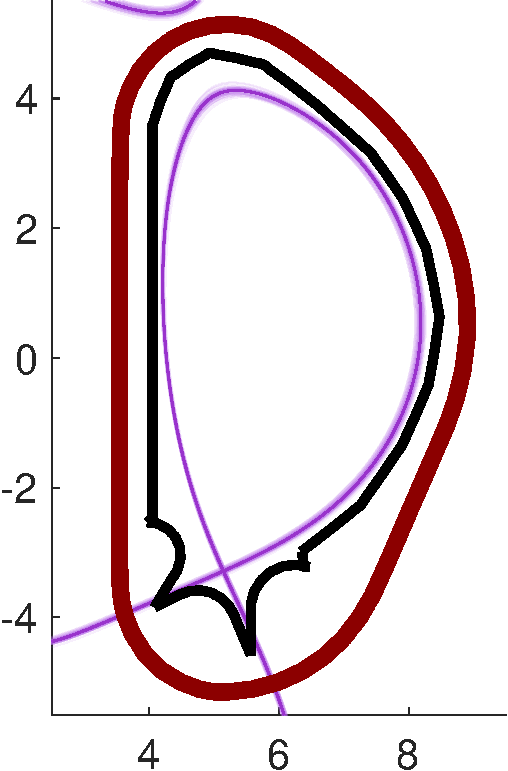
\includegraphics[width=0.19\linewidth]{./figures/QoI_MC_uniform.pdf}
% &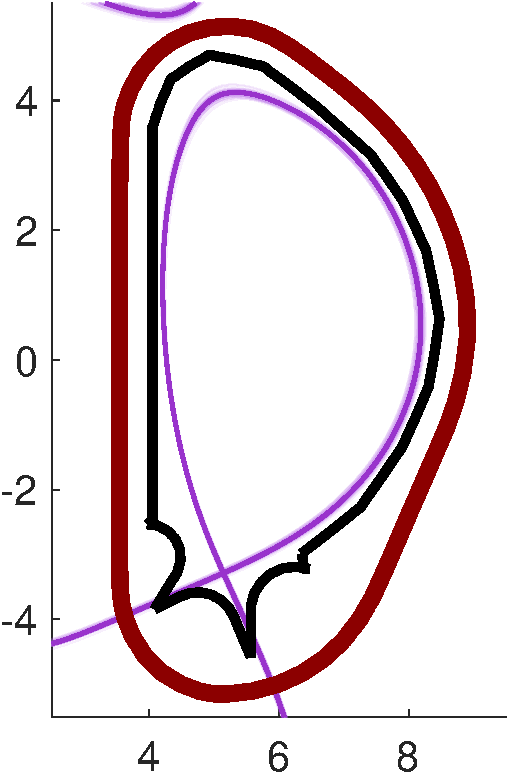
\includegraphics[width=0.19\linewidth]{./figures/QoI_MC_surrogate.pdf}
&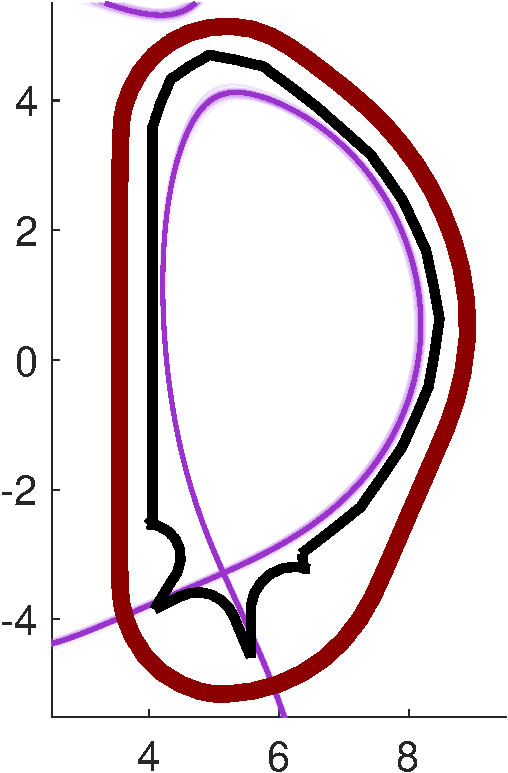
\includegraphics[width=0.19\linewidth]{./figures/QoI_MLMC_DirectSolver_Interp2CommonGrid.pdf} 
& 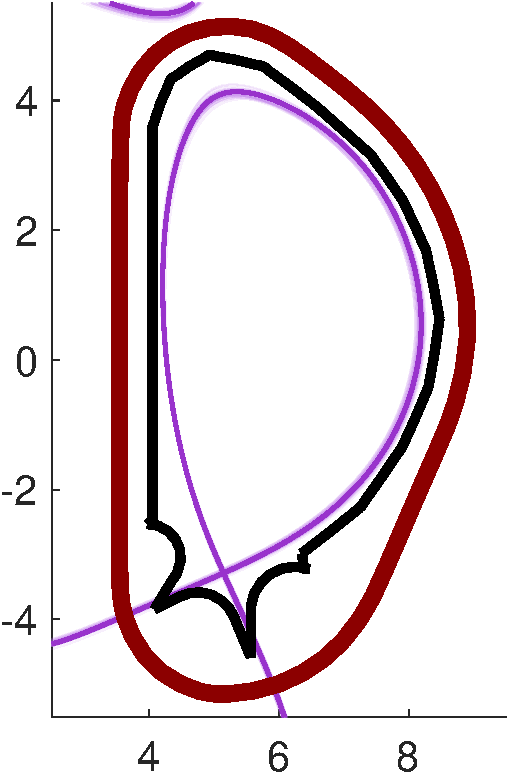
\includegraphics[width=0.19\linewidth]{./figures/QoI_MFMC.pdf} 
\\
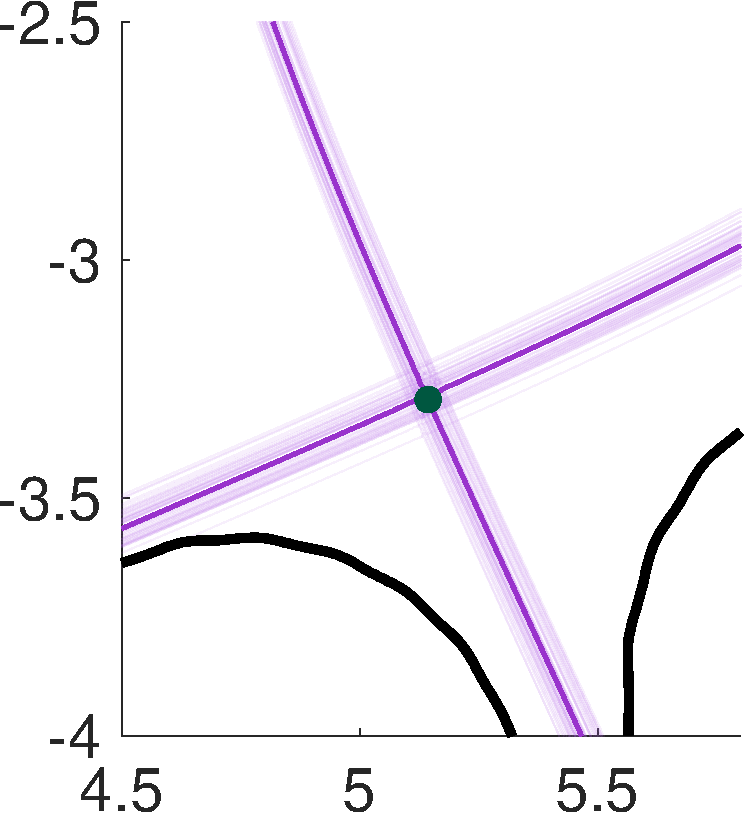
\includegraphics[width=0.19\linewidth]{./figures/QoI_MC_uniform_xptRegion.pdf} 
% &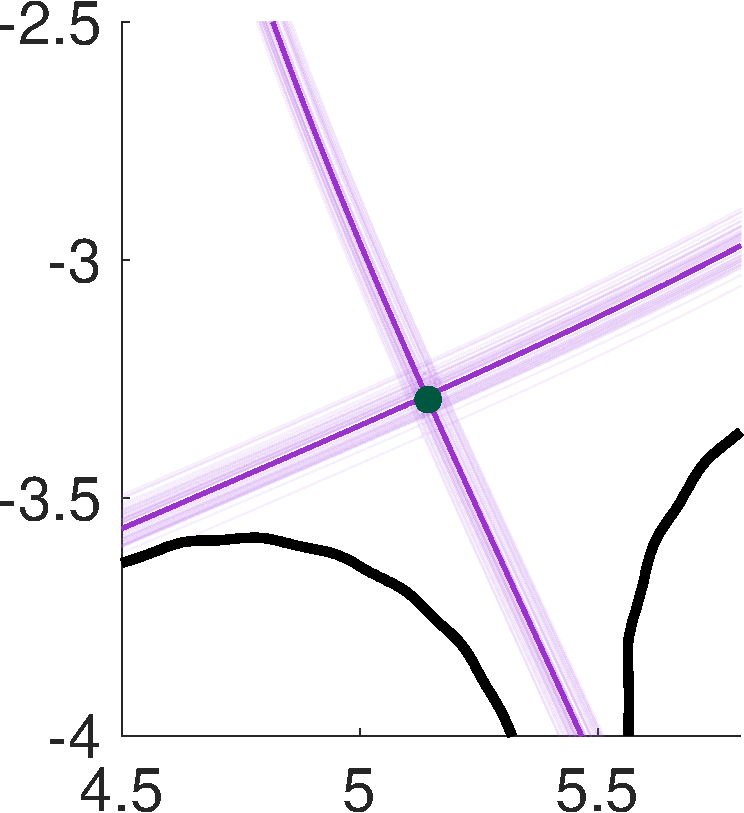
\includegraphics[width=0.19\linewidth]{./figures/QoI_MC_surrogate_xptRegion.pdf}
&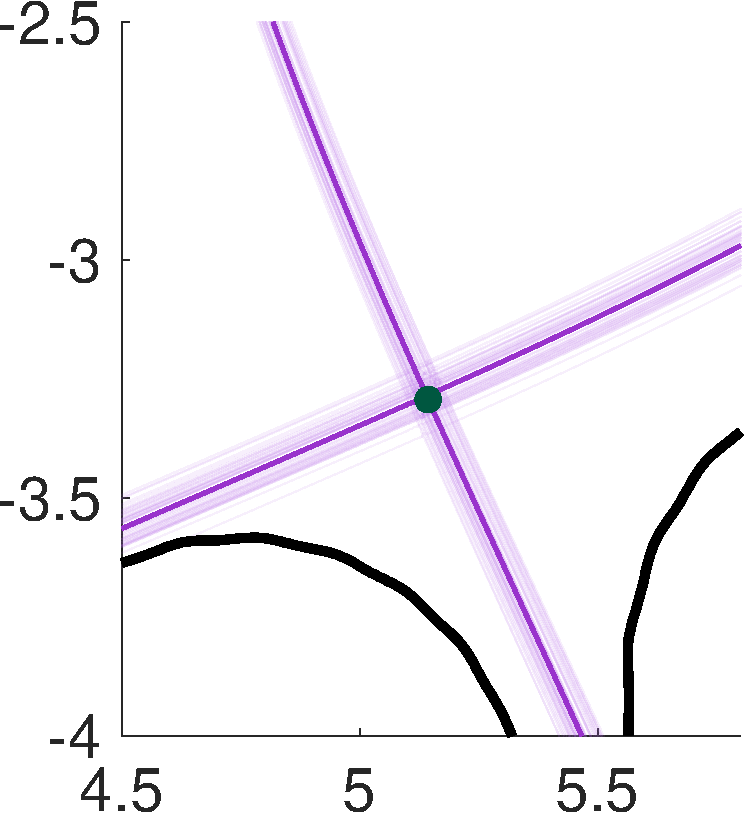
\includegraphics[width=0.19\linewidth]{./figures/QoI_MLMC_DirectSolver_xptRegion_Interp2CommonGrid.pdf} 
&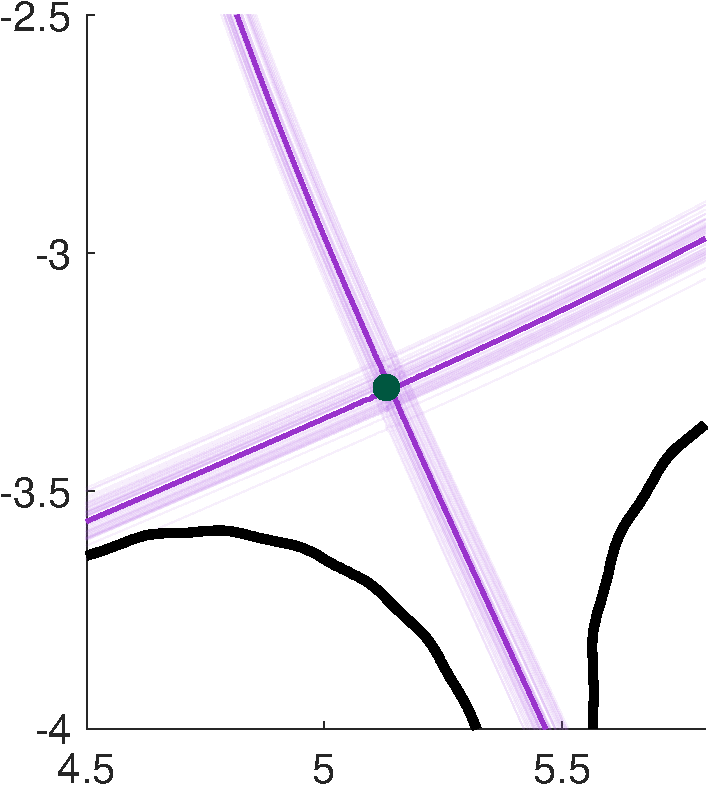
\includegraphics[width=0.19\linewidth]{./figures/QoI_MFMC_xptRegion.pdf} 
\\[1ex]
\quad MC-FE + Direct Solve &MLMC-FE + Direct Solve &MFMC-FE  \\[-0.5ex]
\end{tabular}
\caption{The overlayed plasma boundaries of 50 random realizations are 
displayed in the top row as violet curves (interpolated to the finest mesh with spatial grid level $\ell=4$). The solid violet line is the plasma boundary of the expected 
poloidal flux generated with tolerance $\epsilon=4\times 10^{-4}$. 
The inner and outer walls of the reactor are displayed in solid black and 
dark red respectively. The bottom row shows the regions close to the 
x-points in more detail. The dark green dots are the x-points of the expected 
solution. The columns from left to right correspond to simulations using the 
MC-FE approach with the direct solver and surrogate, MLMC-FE with direct 
solver and surrogate. All simulations were interpolated to the geometry-conforming uniform meshes of discretization level $\ell=4$.} 
\label{fig:QoI_plot}
\end{figure}
%





The sample size estimation for various $\epsilon$ is shown in Table \ref{Tab:SampleSize}.


%
\begin{table}[ht]
	\centering
			\scalebox{0.62}{
   \begin{tabular}{c|c|c|c|c|c|c|c|c|c|c|c|c|}
	    \cline{2-7}	
		&\multicolumn{6}{|c|}{ Level $\ell$}\\
			\hline
			\multicolumn{1}{|c|}{$\epsilon$}&0&1&2&3&4&5\\
			\hline
			\multicolumn{1}{|c|}{$8\times 10^{-3} $}&&&5&&&\\
			\multicolumn{1}{|c|}{$6\times 10^{-3} $}&&&9&&&\\
			\multicolumn{1}{|c|}{$4\times 10^{-3} $}&&&&21&&\\
			\multicolumn{1}{|c|}{$2\times 10^{-3} $}&&&&73&&\\
			\multicolumn{1}{|c|}{$10^{-3} $}&&&&&287&\\
			\multicolumn{1}{|c|}{$8\times 10^{-4} $}&&&&&445&\\
			\multicolumn{1}{|c|}{$6\times 10^{-4} $}&&&&&845&\\
                \multicolumn{1}{|c|}{$4\times 10^{-4} $}&&&&&2000&\\
                \multicolumn{1}{|c|}{$2\times 10^{-4} $}&&&&&& 8000$^{\ast}$\!\!\\
			\hline
	\end{tabular}
 \qquad
		\begin{tabular}{c|c|c|c|c|c|c|c|c|c|c|c|c|}
	    \cline{2-7}	
		&\multicolumn{6}{|c|}{ Level $\ell$}\\
			\hline
			\multicolumn{1}{|c|}{$\epsilon$}&0&1&2&3&4&5\\
			\hline
			\multicolumn{1}{|c|}{$8\times 10^{-3} $}&10     &2     &2&&&\\
			\multicolumn{1}{|c|}{$6\times 10^{-3} $}&12     &2     &2&&&\\
			\multicolumn{1}{|c|}{$4\times 10^{-3} $}&22     &5     &2     &2&&\\
			\multicolumn{1}{|c|}{$2\times 10^{-3} $}&163    &26     &5     &2&&\\
			\multicolumn{1}{|c|}{$10^{-3} $}&577   &90    &15     &3     &2&\\
			\multicolumn{1}{|c|}{$8\times 10^{-4} $}&1036 &157 &26 &5 &2&\\
			\multicolumn{1}{|c|}{$6\times 10^{-4} $}&1744 &266 &44 &9 &2&\\
                \multicolumn{1}{|c|}{$4\times 10^{-4} $}&3911 &553 &86 &17 &4&\\
                \multicolumn{1}{|c|}{$2\times 10^{-4} $}&15619 &2298 &370 &57 &12 &2\\
			\hline
	\end{tabular}
 \qquad
		\begin{tabular}{c|c|c|c|c|c|c|c|c|c|c|c|c|c|c|c|c|c|}
	    \cline{2-7}	
		&\multicolumn{6}{|c|}{ Level $\ell$}\\
			\hline
			\multicolumn{1}{|c|}{$\epsilon$}&0&1&2&3&4&5\\
			\hline
			\multicolumn{1}{|c|}{$8\times 10^{-3} $}&&&&&&\\
			\multicolumn{1}{|c|}{$6\times 10^{-3} $}&&&&&&\\
			\multicolumn{1}{|c|}{$4\times 10^{-3} $}&2&2&2&2&&\\
			\multicolumn{1}{|c|}{$2\times 10^{-3} $}&2&2&2&2&&\\
			\multicolumn{1}{|c|}{$10^{-3} $}&2&2&&2&2&\\
			\multicolumn{1}{|c|}{$8\times 10^{-4} $}&2&2&&2&2&\\
                \multicolumn{1}{|c|}{$6\times 10^{-4} $}&2&2&&2&2&\\
			\multicolumn{1}{|c|}{$4\times 10^{-4} $}&2&2&&2&2&\\
                \multicolumn{1}{|c|}{$2\times 10^{-4} $}&7&2&2&2&2&2\\
			\hline
	\end{tabular}
 
 }
	\caption{The optimal sample size estimation for MC-FE (left), uniform MLMC-FE (middle), and MFMC-FE (right). The simulations were conducted for a variety of choices of $\epsilon$. The computational cost associated with a tolerance of $\epsilon = 2\times 10^{-4}$ for Monte Carlo was prohibitive; the entry in the table for this tolerance (with an asterisk) is an estimate.}
	\label{Tab:SampleSize}
\end{table}
%

%
\begin{table}[ht]
	\centering
			\scalebox{0.62}{
   \begin{tabular}{c|c|c|c|c|c|c|c|c|c|c|c|c|}
			\hline
			\multicolumn{1}{|c|}{ }&MC-FE &MLMC-FE &MFMC-FE\\
			\multicolumn{1}{|c|}{$\epsilon$}&Time & \begin{tabular}{cc} \,\,\,\,\,Time & \,\,\,Speedup \end{tabular}  &\begin{tabular}{cc} \,\,\,\,Time & \,\,\,Speedup \end{tabular}\\
			\hline
			\multicolumn{1}{|c|}{$8\times 10^{-3} $}&1.42e+01&\begin{tabular}{cc}6.61e+00\,\,\, & 2.1 \end{tabular}&\begin{tabular}{cc}..\,\,  & .. \end{tabular} \\
			\multicolumn{1}{|c|}{$6\times 10^{-3} $}&2.75e+01&\begin{tabular}{cc}7.44e+00\,\,\, & 3.7 \end{tabular}&\begin{tabular}{cc}..\,\, &.. \end{tabular}\\
			\multicolumn{1}{|c|}{$4\times 10^{-3} $}&6.60e+01&\begin{tabular}{cc}4.36e+01\,\,\, & 1.5 \end{tabular}&\begin{tabular}{cc}..& .. \end{tabular}\\
			\multicolumn{1}{|c|}{$2\times 10^{-3} $}&2.19e+02&\begin{tabular}{cc}4.73e+01\,\, & 4.6\end{tabular}&\begin{tabular}{cc}..& .. \end{tabular}\\
			\multicolumn{1}{|c|}{$10^{-3} $}&4.66e+03&\begin{tabular}{cr}1.66e+02\,\, & 28.1 \end{tabular}&\begin{tabular}{cc}..& .. \end{tabular}\\
			\multicolumn{1}{|c|}{$8\times 10^{-4} $}&8.02e+03&\begin{tabular}{cc}4.33e+02\,\, & 18.5 \end{tabular}&\begin{tabular}{cc}..& ..
            \end{tabular}\\
			\multicolumn{1}{|c|}{$6\times 10^{-4} $}&1.49e+04&\begin{tabular}{cc}5.36e+02\,\, & 27.8 \end{tabular}&\begin{tabular}{cc}.. & .. \end{tabular}\\
                \multicolumn{1}{|c|}{$4\times 10^{-4} $}&3.66e+04&\begin{tabular}{cc}1.03e+03\,\, & 35.4 \end{tabular} &\begin{tabular}{cc}..& .. \end{tabular}\\
                \multicolumn{1}{|c|}{$2\times 10^{-4} $}&5.84e+05$^{\ast}$\!\!\!&\begin{tabular}{cc}4.90e+03 &119.2 \end{tabular} &\begin{tabular}{cc}..&.. \end{tabular}\\
			\hline
	\end{tabular}
 }
	\caption{The CPU time in seconds for MC-FE (left), uniform MLMC-FE (middle), and MFMC-FE (right), together with speedups for the multilevel methods, for a variety of choices of $\epsilon$. The computational cost associated with a tolerance of $\epsilon = 2\times 10^{-4}$ for Monte Carlo was prohibitive; the entry in the table for this tolerance (with an asterisk) is an estimate.}
	\label{Tab:CPU_time}
\end{table}
%




\noindent \textbf{Geometric descriptors.}
%
\begin{table}[ht]
	\centering
			\scalebox{0.6}{
		\begin{tabular}{c|c|c|c|c|c|c|}
			\cline{2-5}
				&\multicolumn{1}{c|}{MC-FE DS}&MLMC-FE DS&MLMC-FE DS (Interp)&MLMC-FE Surrogate (Interp)\\
			\hline
			\multicolumn{1}{|c|}{x point}&(5.14,-3.29)&(5.14,-3.29)&(5.14,-3.29)&(5.14,-3.29)\\
			\hline
			\multicolumn{1}{|c|}{magnetic axis}&(6.41,0.61)&(6.44,0.56)&(6.41,0.61)&(6.41,0.61)\\
			\hline
			\multicolumn{1}{|c|}{strike} &(4.16,-3.71)&(4.16,-3.71)&(4.16,-3.71)&(4.16,-3.71)\\
			\multicolumn{1}{|c|}{points}&(5.56,-4.22)&(5.56,-4.22)&(5.56,-4.22)&(5.56,-4.22)\\
			\hline
			\multicolumn{1}{|c|}{inverse aspect ratio} &0.32&0.32&0.32&0.32\\
			\hline
			\multicolumn{1}{|c|}{elongation} &1.86&1.87&1.86&1.86\\
			\hline
			\multicolumn{1}{|c|}{upper triangularity}&0.43&0.43&0.43&0.43\\
			\hline
			\multicolumn{1}{|c|}{lower triangularity} &0.53&0.53&0.53&0.53\\
			\hline
	\end{tabular}
  }
	\caption{Geometric parameters of the expected poloidal flux $u$ from MC-FE with direct solver, MLMC-FE with direct solver,  MLMC-FE with direct solver with interpolating solution to a common fine grid of level $L=5$, MLMC-FE with surrogate with interpolating solution to a common fine grid of level $L=5$. The results are generated with an nMSE $4\times 10^{-4}$ on the geometry-conforming uniform mesh set.}
	\label{Tab: QoI_GeoInfo}
\end{table}






% % =============================
% \subsection{Uncertainties in the source term}
% % =============================
% In this experiment, we study the uncertainty in perturbing the reference parameter that characterizes the source term \eqref{eq:source}.
% \begin{table}[ht]
% 	\centering
% 			\scalebox{0.62}{
%    \begin{tabular}{c|c|c|c|c|c|c|c|c|c|c|c|c|}
% 	    \cline{2-7}	
% 		&\multicolumn{6}{|c|}{ Level $\ell$}\\
% 			\hline
% 			\multicolumn{1}{|c|}{$\epsilon$}&0&1&2&3&4&5\\
% 			\hline
% 			\multicolumn{1}{|c|}{$8\times 10^{-3} $}&&&8&&&\\
% 			\multicolumn{1}{|c|}{$6\times 10^{-3} $}&&&10&&&\\
% 			\multicolumn{1}{|c|}{$4\times 10^{-3} $}&&&&25&&\\
% 			\multicolumn{1}{|c|}{$2\times 10^{-3} $}&&&&93&&\\
% 			\multicolumn{1}{|c|}{$10^{-3} $}&&&&&423&\\
% 			\multicolumn{1}{|c|}{$8\times 10^{-4} $}&&&&&678&\\
% 			\multicolumn{1}{|c|}{$6\times 10^{-4} $}&&&&&1211&\\
%                 \multicolumn{1}{|c|}{$4\times 10^{-4} $}&&&&&2700$^{\ast}$&\\
%                 \multicolumn{1}{|c|}{$2\times 10^{-4} $}&&&&&&11000$^{\ast}$\!\!\\
% 			\hline
% 	\end{tabular}
%  \qquad
% 		\begin{tabular}{c|c|c|c|c|c|c|c|c|c|c|c|c|}
% 	    \cline{2-7}	
% 		&\multicolumn{6}{|c|}{ Level $\ell$}\\
% 			\hline
% 			\multicolumn{1}{|c|}{$\epsilon$}&0&1&2&3&4&5\\
% 			\hline
% 			\multicolumn{1}{|c|}{$8\times 10^{-3} $}&10 &2 &2&&&\\
% 			\multicolumn{1}{|c|}{$6\times 10^{-3} $}&11 &3 &2 &&&\\
% 			\multicolumn{1}{|c|}{$4\times 10^{-3} $}&33 &7 &2 &2&&\\
% 			\multicolumn{1}{|c|}{$2\times 10^{-3} $}&150 &27 &4 &2&&\\
% 			\multicolumn{1}{|c|}{$10^{-3} $}&692 &116 &19 &4 &2&\\
% 			\multicolumn{1}{|c|}{$8\times 10^{-4} $}&1008 &160 &27 &6 &2&\\
% 			\multicolumn{1}{|c|}{$6\times 10^{-4} $}&2022 &322 &53 &10 &3&\\
%                 \multicolumn{1}{|c|}{$4\times 10^{-4} $}&4158 &613 &106 &14 &4&\\
%                 \multicolumn{1}{|c|}{$2\times 10^{-4} $}&17158 &2612 &442 &59 &13 &2\\
% 			\hline
% 	\end{tabular}
%  \qquad
% 		\begin{tabular}{c|c|c|c|c|c|c|c|c|c|c|c|c|c|c|c|c|c|}
% 	    \cline{2-7}	
% 		&\multicolumn{6}{|c|}{ Level $\ell$}\\
% 			\hline
% 			\multicolumn{1}{|c|}{$\epsilon$}&0&1&2&3&4&5\\
% 			\hline
% 			\multicolumn{1}{|c|}{$8\times 10^{-3} $}&&&&&&\\
% 			\multicolumn{1}{|c|}{$6\times 10^{-3} $}&&&&&&\\
% 			\multicolumn{1}{|c|}{$4\times 10^{-3} $}&&&\\
% 			\multicolumn{1}{|c|}{$2\times 10^{-3} $}&&&\\
% 			\multicolumn{1}{|c|}{$10^{-3} $}&&&&&&\\
% 			\multicolumn{1}{|c|}{$8\times 10^{-4} $}&&&&&&\\
%                 \multicolumn{1}{|c|}{$6\times 10^{-4} $}&&&&&&\\
% 			\multicolumn{1}{|c|}{$4\times 10^{-4} $}&&&&&&\\
%                 \multicolumn{1}{|c|}{$2\times 10^{-4} $}&&&&&&\\
% 			\hline
% 	\end{tabular}
 
%  }
% 	\caption{The optimal sample size estimation for MC-FE (left), uniform MLMC-FE (middle), and MFMC-FE (right). The simulations were conducted for a variety of choices of $\epsilon$. The computational cost associated with a tolerance of $\epsilon = 2\times 10^{-4}$ for Monte Carlo was prohibitive; the entry in the table for this tolerance (with an asterisk) is an estimate.}
% 	\label{Tab:SampleSize_Source_Term}
% \end{table}

% \begin{table}[ht]
% 	\centering
% 			\scalebox{0.62}{
%    \begin{tabular}{c|c|c|c|c|c|c|c|c|c|c|c|c|}
% 			\hline
% 			\multicolumn{1}{|c|}{ }&MC-FE &MLMC-FE &MFMC-FE\\
% 			\multicolumn{1}{|c|}{$\epsilon$}&Time & \begin{tabular}{cc} \,\,\,\,\,Time & \,\,\,Speedup \end{tabular}  &\begin{tabular}{cc} \,\,\,\,Time & \,\,\,Speedup \end{tabular}\\
% 			\hline
% 			\multicolumn{1}{|c|}{$8\times 10^{-3} $}&9.71e+01&\begin{tabular}{cc}1.10e+01\,\,\, & 8.8 \end{tabular}&\begin{tabular}{cc}..\,\,  & .. \end{tabular} \\
% 			\multicolumn{1}{|c|}{$6\times 10^{-3} $}&1.16e+02&\begin{tabular}{cc}1.27e+01\,\,\, & 9.1 \end{tabular}&\begin{tabular}{cc}..\,\, &.. \end{tabular}\\
% 			\multicolumn{1}{|c|}{$4\times 10^{-3} $}&1.29e+02&\begin{tabular}{cc}3.39e+01\,\,\, & 3.8 \end{tabular}&\begin{tabular}{cc}..& .. \end{tabular}\\
% 			\multicolumn{1}{|c|}{$2\times 10^{-3} $}&8.03e+02&\begin{tabular}{cc}7.29e+01\,\, & 11.0\end{tabular}&\begin{tabular}{cc}..& .. \end{tabular}\\
% 			\multicolumn{1}{|c|}{$10^{-3} $}&1.49e+04&\begin{tabular}{cr}2.55e+02\,\, & 58.5 \end{tabular}&\begin{tabular}{cc}..& .. \end{tabular}\\
% 			\multicolumn{1}{|c|}{$8\times 10^{-4} $}&3.89e+04&\begin{tabular}{cc}2.76e+02\,\, &140.6 \end{tabular}&\begin{tabular}{cc}..& ..
%             \end{tabular}\\
% 			\multicolumn{1}{|c|}{$6\times 10^{-4} $}&1.1219e+05&\begin{tabular}{cc}7.1946e+02\,\, & .. \end{tabular}&\begin{tabular}{cc}.. & .. \end{tabular}\\
%                 \multicolumn{1}{|c|}{$4\times 10^{-4} $}&..&\begin{tabular}{cc}1.1598e+03\,\, & .. \end{tabular} &\begin{tabular}{cc}..& .. \end{tabular}\\
%                 \multicolumn{1}{|c|}{$2\times 10^{-4} $}&..$^{\ast}$\!\!\!&\begin{tabular}{cc}4.4956e+03 &.. \end{tabular} &\begin{tabular}{cc}..&.. \end{tabular}\\
% 			\hline
% 	\end{tabular}
%  }
% 	\caption{The CPU time in seconds for MC-FE (left), uniform MLMC-FE (middle), and MFMC-FE (right), together with speedups for the multilevel methods, for a variety of choices of $\epsilon$. The computational cost associated with a tolerance of $\epsilon = 2\times 10^{-4}$ for Monte Carlo was prohibitive; the entry in the table for this tolerance (with an asterisk) is an estimate.}
% 	\label{Tab:CPU_time_Source_Term}
% \end{table}